\section{Vorlesung 04.05.2016}
\subsection{Begriffe}

\textbf{Vertebraten:}\footnote{\url{https://de.wikipedia.org/wiki/Wirbeltiere}} Wirbeltiere (Vertebrata) sind Tiere, die eine Wirbelsäule besitzen. Zu den Vertebraten gehören fünf klassische Großgruppen: Säugetiere, Vögel, Reptilien, Amphibien sowie Fische (Knochen- und Knorpelfische), als urtümliche Vertreter zudem die Rundmäuler.
\\\\
\textbf{Invertebraten:}\footnote{\url{https://de.wikipedia.org/wiki/Wirbellose}} Wirbellose, Invertebrata oder Evertebrata sind vielzellige Tiere ohne Wirbelsäule. Zu dieser informellen Gruppe (Formtaxon) von Lebewesen gehört die Mehrzahl aller bekannten Tierarten.
\\\\
\textbf{Nervenzelle:}\footnote{\url{https://de.wikipedia.org/wiki/Nervenzelle}} Eine Nervenzelle oder ein Neuron ist eine auf Erregungsleitung und Erregungsübertragung spezialisierte Zelle, die als Zelltyp in Gewebetieren und damit in nahezu allen vielzelligen Tieren vorkommt. Die Gesamtheit aller Nervenzellen eines Tieres bildet zusammen mit den Gliazellen das Nervensystem.\\
Eine typische Säugetier-Nervenzelle hat einen Zellkörper und Zellfortsätze zweierlei Art: die Dendriten und den Neuriten bzw. das Axon. Die verästelten Dendriten nehmen vornehmlich Erregung von anderen Zellen auf. Der Neurit eines Neurons, von Gliazellen umhüllt sein Axon, kann über einen Meter lang sein und dient zunächst der Fortleitung einer Erregung dieser Zelle in die Nähe anderer Zellen. Dabei wird eine Spannungsänderung über den Fortsatz weitergeleitet, indem kurzzeitige Ionenströme durch besondere Kanäle in der Zellmembran zugelassen werden.
Die Axonenden stehen über Synapsen, an denen die Erregung selten unmittelbar elektrisch weitergegeben, sondern meist mittels Botenstoffen (Neurotransmittern) chemisch übertragen wird, in Kontakt zu anderen Nervenzellen, Muskelzellen (neuromuskuläre Endplatte) oder zu Drüsenzellen.
\\\\
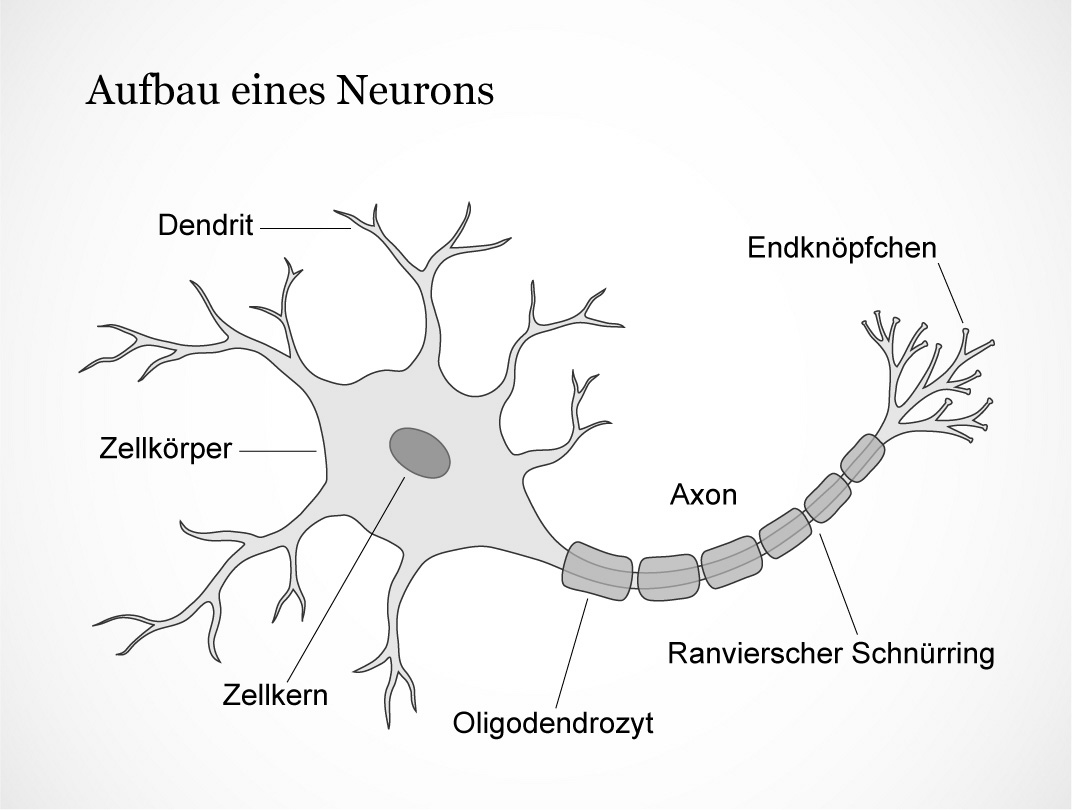
\includegraphics[width=0.6\textwidth]{lectures/160405/pix/neuron.jpg}

\textbf{Axon:}\footnote{\url{https://de.wikipedia.org/wiki/Axon}} Das Axon, selten der Axon, auch Neuraxon oder Achsenzylinder genannt, ist ein oft langer schlauchartiger Nervenzellfortsatz, ein Neurit, der in einer Hülle von Gliazellen verläuft und zusammen mit dieser Umhüllung als Nervenfaser bezeichnet wird. Seitliche Abzweigungen des Axons werden auch dessen Kollaterale genannt und können sich wie das terminale Axon in mehrere Endästchen aufzweigen. Die meisten Neuronen haben ein einziges Axon. Es gibt aber auch Nervenzellen, die kein Axon besitzen, z. B. verschiedene Amakrinzellen der Netzhaut.
\\\\
\textbf{Dendriten:}\footnote{\url{https://de.wikipedia.org/wiki/Dendrit_\%28Biologie\%29}} Dendriten heißen in der Biologie Zellfortsätze von Nervenzellen, die aus dem Zellkörper hervorgehen und vorwiegend der Reizaufnahme dienen. Eine Nervenzelle besteht typischerweise aus drei Anteilen: dem Zellkörper, Soma oder Perikaryon genannt, und Zellfortsätzen, die Dendriten einerseits und der Neurit – in Gliahülle das Axon – andererseits. Es gibt auch spezialisierte Neuronen, die kein Axon haben (z. B. die Amakrinzellen der Netzhaut) oder die keine Dendriten besitzen (z. B. die Stäbchen und Zapfen der Netzhaut) oder solche, bei denen der Zellkörper nicht mehr zwischen Dendritenstamm und Axon liegt und die Fortsätze so ineinander übergehen (pseudouniploare wie bei den sensiblen Spinalganglienzellen).
\\
Nervenzellen werden morphologisch nach der Anzahl ihrer Fortsätze unterschieden:
1: unipolare Nervenzelle, 2: bipolare Nervenzelle, 3: multipolare Nervenzelle, 4: pseudounipolare Nervenzelle\\
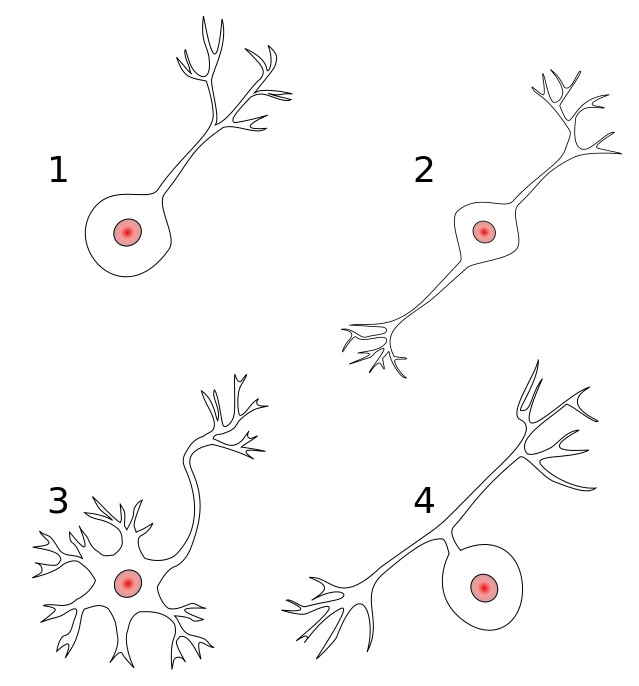
\includegraphics[width=0.6\textwidth]{lectures/160405/pix/dendrite.jpg}
\\\\
\textbf{Synapse:}\footnote{\url{https://de.wikipedia.org/wiki/Synapse}} Synapse bezeichnet die Stelle einer neuronalen Verknüpfung, über die eine Nervenzelle in Kontakt zu einer anderen Zelle steht – einer Sinneszelle, Muskelzelle, Drüsenzelle oder anderen Nervenzellen. Synapsen dienen der Übertragung von Erregung, erlauben aber auch die Modulation der Signalübertragung, und sie vermögen darüber hinaus durch anpassende Veränderungen Information zu speichern. Die Anzahl der Synapsen beträgt im Gehirn eines Erwachsenen etwa 100 Billionen (1014) – bezogen auf ein einzelnes Neuron schwankt sie zwischen 1 und 200.000.
\\\\
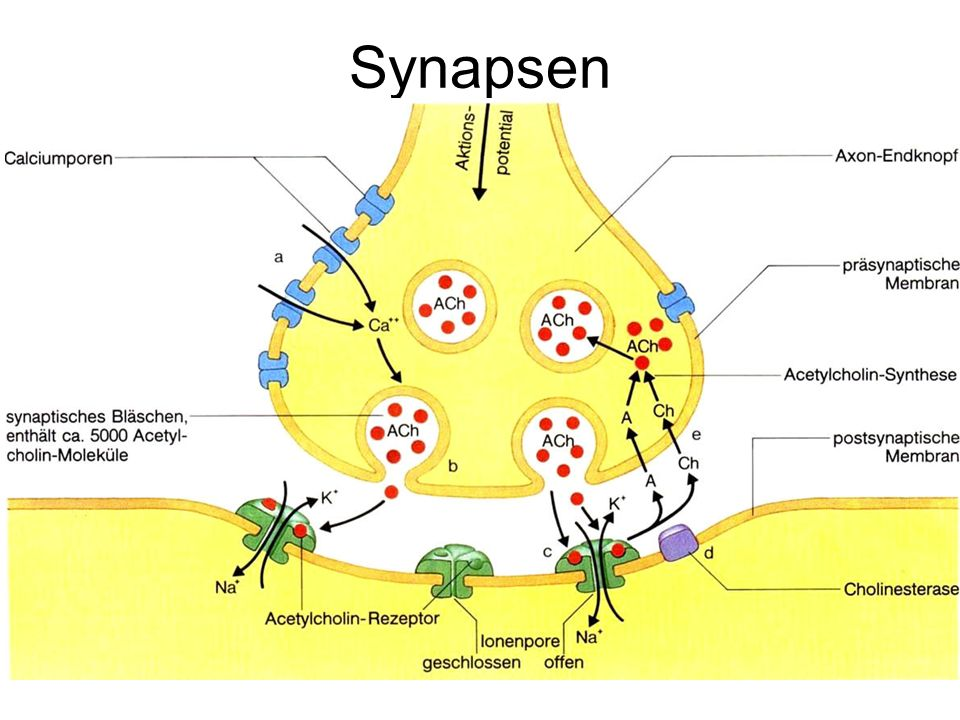
\includegraphics[width=0.95\textwidth]{lectures/160405/pix/synapse.jpg}
In den meisten Fällen sind es chemische Synapsen. Bei ihnen wird das Signal, das als elektrisches Aktionspotential ankommt, in ein chemisches Signal umgewandelt, in dieser Form über den zwischen den Zellen bestehenden synaptischen Spalt getragen, und dann wieder in ein elektrisches Signal umgebildet. Dabei schüttet die sendende Zelle (präsynaptisch) Botenstoffe aus, Neurotransmitter, die sich auf der anderen Seite des Spaltes (postsynaptisch) an Membranrezeptoren der empfangenden Zelle binden. Hierdurch ist die Richtung der Signalübertragung (nur vorwärts) anatomisch festgelegt, was für die Verarbeitung von Information in neuronalen Netzen grundlegend ist. Der erregungsübertragende Transmitter wird entweder in der Endigung des Axons des sendenden Neurons gebildet oder in dessen Zellkörper synthetisiert und axonal zu den präsynaptischen Membranregionen transportiert.
Dagegen sind elektrische Synapsen als gap junctions Kontaktstellen, bei denen Ionenkanäle zweier Zellen unmittelbar aneinander koppeln und so einen Übergang von Ionen und kleinen Molekülen von einer Zelle zur anderen erlauben. Zuerst wurden solche Synapsen zwischen Neuronen entdeckt, doch kommen ähnliche Kontaktstellen noch in anderen Geweben vor, auch in Pflanzen.
In übertragenem Sinn werden als immunologische Synapsen die Stellen vorübergehender zellulärer Kontakte von Zellen des Immunsystems bezeichnet, sowohl untereinander als auch mit Zellen des umgebenden Gewebes. Dabei binden Moleküle auf der Oberfläche der einen Zelle an Rezeptormoleküle und Adhäsionsmoleküle in der Zellmembran der anderen und tauschen darüber Informationen aus.
\\\\
\textbf{Vesikel:}\footnote{\url{https://de.wikipedia.org/wiki/Vesikel_\%28Biologie\%29}} Vesikel (lat. vesicula - Bläschen) in der Biologie sind intrazelluläre (in der Zelle gelegene), sehr kleine, rundliche bis ovale Bläschen, die von einer einfachen oder doppelten Membran oder einer netzartigen Hülle aus Proteinen umgeben sind. Die Vesikel bilden eigene Zellkompartimente, in denen unterschiedliche zelluläre Prozesse ablaufen. Ihre Größe beträgt etwa ein Mikrometer. Vesikel sind für den Transport vieler Stoffe in der Zelle verantwortlich.
\\\\
\textbf{Gliazelle:}\footnote{\url{https://de.wikipedia.org/wiki/Gliazelle}} Gliazelle ist ein Sammelbegriff für strukturell und funktionell von den Nervenzellen (Neuronen) abgrenzbare Zellen im Nervengewebe. Nach heutigen Erkenntnissen bilden Gliazellen nicht nur ein Stützgerüst für Nervenzellen, sondern sorgen auch durch ihre Umhüllung für deren elektrische Isolation. Weiterhin sind Gliazellen maßgeblich an Stofftransport und Flüssigkeitsaustausch sowie an der Aufrechterhaltung der Homöostase im Gehirn beteiligt. Darüber hinaus wirken sie auch im Prozess der Informationsverarbeitung, -speicherung und -weiterleitung mit.
Etwa die Hälfte der Zellen im menschlichen Gehirn sind Gliazellen, ähnlich wie bei anderen Primaten. Gliazellen sind meist kleiner als die Nervenzellen, im Unterschied zu diesen variiert ihre durchschnittliche Zellmasse im Nervengewebe nur gering bei verschiedenen Säugetierspezies. In deren Hirnstrukturen hängt das jeweilige Verhältnis von Glia zu Neuronen nach Anzahl und Volumen hauptsächlich von der durchschnittlichen Neuronengröße ab.
\\\\
\textbf{Myelinisierung:}\footnote{\url{https://de.wikipedia.org/wiki/Nervenfaser}} Myelinisierung wird die mehrfache Umwicklung des Neuriten einer Nervenzelle durch umhüllende Gliazellen genannt, wodurch das Axon elektrisch derart isoliert wird, dass mit Umbau seiner Internodien eine schnellere Erregungsleitung möglich wird.
\\\\
\textbf{Neurotransmitter:}\footnote{\url{https://de.wikipedia.org/wiki/Neurotransmitter}} Neurotransmitter sind Botenstoffe, die an chemischen Synapsen die Erregung von einer Nervenzelle auf andere Zellen übertragen (synaptische Transmission). Die Neurotransmitter werden im Zellkörper oder in der Endigung des Axons vom sendenden Neuron synthetisiert und in Quanten freigesetzt.